%!TeX program = xelatex
%!TeX encoding = UTF-8 Unicode
% A20OS 决赛答辩幻灯片 —— 自定义主题 a20beamer（docs/slides/a20beamer.sty）
% 编译（在 docs/ 目录下）：
%   TEXINPUTS="slides:" xelatex slides.tex && TEXINPUTS="slides:" xelatex slides.tex
\documentclass[aspectratio=1610]{beamer}

% ==================== 基本信息 ====================
\title{A20OS：高性能混合内核操作系统}
\subtitle{从 MCU 到完整桌面：双重 ABI · 八大平台 · 工程化并发安全}
\author{AAAAAAAAAAAAAAAAAAAA} % TODO: 替换为参赛队名/队员
\institute{武汉大学}
\date{2026 年 8 月}

% ==================== 自定义主题 ====================
\usepackage{a20beamer}
\graphicspath{{slides/figures/}{figures/}}

% 代码块风格
\usepackage{listings}
\lstdefinestyle{a20c}{
    language=C,
    numbers=left,
    numberstyle=\tiny\color{a20gray},
    basicstyle=\ttfamily\scriptsize,
    keywordstyle=\bfseries\color{a20blue},
    commentstyle=\itshape\color{a20gray},
    stringstyle=\color{a20amber!80!black},
    breaklines=true,
    tabsize=4,
    showstringspaces=false,
    xleftmargin=1.5em,
    frame=none
}
\lstset{escapechar=@, style=a20c}

% 截图占位：figures/<name> 存在则用真图，否则显示占位框
\newcommand{\shotslot}[2]{%
    \begin{tcolorbox}[colback=white, colframe=a20navy!30, arc=1mm, boxrule=0.6pt,
                      left=1pt, right=1pt, top=1pt, bottom=1pt]
        \IfFileExists{figures/#1}{%
            \includegraphics[width=\linewidth]{#1}%
        }{%
            \begin{minipage}[c][0.19\paperheight][c]{\linewidth}
                \centering\color{a20gray}\scriptsize
                预留截图位\\[0.4em]\ttfamily\footnotesize #1
            \end{minipage}%
        }%
    \end{tcolorbox}
    \vspace{0.1em}
    {\scriptsize\color{a20gray}#2\par}}

\begin{document}

\begin{frame}[plain]
    \titlepage
\end{frame}

% ==================== 目录 ====================
\begin{frame}{目录}
    \small
    \begin{columns}[t]
        \begin{column}{0.48\textwidth}
            \tableofcontents[sections={1-7},hideallsubsections]
        \end{column}
        \begin{column}{0.48\textwidth}
            \tableofcontents[sections={8-13},hideallsubsections]
        \end{column}
    \end{columns}
\end{frame}

% ==================================================
\renewcommand{\azsectionsummary}{%
    \statcard[0.23\linewidth]{19.2 万}{自研代码行数}\hfill
    \statcard[0.23\linewidth]{500}{双 ABI syscall（361 + 139）}\hfill
    \statcard[0.23\linewidth]{8}{指令集架构}\hfill
    \statcard[0.23\linewidth]{483}{次提交 / 20 周连续演进}}
\section{项目概览}

\begin{frame}{A20OS 是什么？—— 一页看完成度}
    \begin{columns}[t]
        \begin{column}{0.62\textwidth}
            \footnotesize
            \begin{itemize}
                \item \high{混合内核}：性能路径留内核，易崩服务迁用户态
                \item \high{双重 ABI}：361 Linux syscall 兼容 + 139 Native syscall
                \item \high{八大平台}：7 hosted + ARMv7-M；星光 2 / LS2K1000 / STM32
                \item \high{完整桌面}：Wayland + LVGL 自研桌面 + virtio-gpu 3D
                \item \high{工程化}：锁契约文档化、54 项冒烟门禁、七架构矩阵
            \end{itemize}
            \vspace{0.2em}
            \begin{a20keybox}
                \footnotesize 同一内核：从 64\,KiB Flash 的 MCU，跑到 Alpine 发行版桌面。
            \end{a20keybox}
        \end{column}
        \begin{column}{0.36\textwidth}
            \statcard[0.98\linewidth]{180/180}{BuildStorm 用例全过（双架构）}
            \vspace{0.3em}
            \statcard[0.98\linewidth]{54}{项行为冒烟门禁（\code{make smoke-*}）}
            \vspace{0.3em}
            \statcard[0.98\linewidth]{92 篇}{设计文档，1.6 万行，随码同仓}
        \end{column}
    \end{columns}
\end{frame}

\begin{frame}{从初赛到决赛：能力跃迁}
    \begin{table}
        \centering
        \footnotesize
        \renewcommand{\arraystretch}{1.18}
        \begin{tabular}{lll}
            \toprule
            \textbf{维度} & \textbf{初赛} & \textbf{决赛（当前）} \\
            \midrule
            内核规模 & 约 18 万行 / 800+ 文件 & \high{22.2 万行 / 982 文件}（自研 15.7 万） \\
            支持架构 & 4 个 & \high{7 hosted + ARMv7-M MCU} \\
            Linux ABI & 部分 syscall & \high{361 全表覆盖}，含 io\_uring / landlock / mseal \\
            Native ABI & 90 syscall & \high{139 syscall} + Pager / monitor 深化 \\
            调度器 & 8 级 MLFQ & \high{EEVDF} + per-CPU 队列 + 空闲窃取 \\
            桌面 / 发行版 & -- & \high{Wayland 桌面 + 3D} / Alpine rootfs 直跑 \\
            混合内核服务 & -- & \high{svcmgr / 用户态驱动 / KEP 扩展} \\
            BuildStorm 耗时 & 2551 s / 2315 s（RV / LA） & \high{1483 s / 1399 s}（\good{-42\% / -40\%}） \\
            \bottomrule
        \end{tabular}
    \end{table}
    \vspace{0.2em}
    \begin{center}
        \small 从“能启动、能跑几个程序”进化到\high{可跑完整桌面与发行版、可跑决赛高性能负载}的通用内核。
    \end{center}
\end{frame}

\begin{frame}{从零开始：不基于任何现有内核}
    \begin{columns}[t]
        \begin{column}{0.56\textwidth}
            \footnotesize
            \begin{itemize}
                \item \high{首个 commit}（2026-04-11）：8,052 行最小内核 + 基础用户程序；此后 \high{483 次提交、20 周连续演进}
                \item \high{无一次性导入}：最大单 commit 即首个最小内核，其余全部是 $\le$ 7.5k 行的增量功能提交
                \item \high{内核树零 submodule}：23 个 submodule 全部是用户态应用 / 库 / 工具链（vim、git、LVGL 等），隔离于 \code{user/external/}
                \item 内核唯一第三方组件：\high{lwIP 协议栈}，目录级隔离于 \code{kernel/external/}，不计入自研工作量
                \item 非衍生自 Linux / xv6 / rCore / FreeRTOS / RT-Thread / ArceOS 等任何现有内核
            \end{itemize}
            \vspace{0.2em}
            \srcnote{证据即仓库：\code{git log --reverse} 逐 commit 可查；第三方边界有编译期门禁审查}
        \end{column}
        \begin{column}{0.41\textwidth}
            \begin{tikzpicture}[baseline={(current bounding box.north)}]
                \begin{axis}[
                    xbar stacked, xmin=0, xmax=27.5,
                    width=0.98\linewidth, height=2.1cm,
                    ytick=\empty,
                    xmajorgrids, major grid style={a20navy!10},
                    axis line style={draw=none}, tick style={draw=none},
                    xticklabel style={font=\tiny, color=a20gray},
                    xlabel={代码构成（万行）}, xlabel style={font=\scriptsize},
                    bar width=17pt,
                ]
                    \addplot[xbar, fill=a20blue, draw=none] coordinates {(15.7,0)};
                    \addplot[xbar, fill=a20accent, draw=none] coordinates {(3.5,0)};
                    \addplot[xbar, fill=a20gray!45, draw=none] coordinates {(6.5,0)};
                \end{axis}
            \end{tikzpicture}
            \vspace{-0.4em}
            \begin{center}
                \tiny\textcolor{a20blue}{■} 自研内核 15.7 万 ~\textcolor{a20accent}{■} 自研用户态 3.5 万 ~\textcolor{a20gray}{■} lwIP（隔离）6.5 万
            \end{center}
            \vspace{0.3em}
            \begin{a20keybox}
                \footnotesize 内核主干 \high{100\% 自研}；另含 \high{18 个}编译期注册驱动、\high{53 个}自研用户态命令 / 测试程序。
            \end{a20keybox}
        \end{column}
    \end{columns}
\end{frame}

\begin{frame}{20 周、483 次提交：从 8k 行最小内核到 16 万行内核}
    \begin{columns}[t]
        \begin{column}{0.63\textwidth}
            \begin{tikzpicture}[baseline={(current bounding box.north)}]
                \pgfplotsset{set layers}
                \begin{axis}[
                    width=0.99\linewidth, height=5.0cm, scale only axis,
                    xmin=0.5, xmax=20.5, ymin=0, ymax=150,
                    axis y line*=right, hide x axis,
                    ytick=\empty,
                    tick style={draw=none},
                ]
                    \addplot[ybar, bar width=4pt, fill=a20accent!40, draw=none] coordinates {
                        (1,1)(2,16)(3,7)(4,8)(5,9)(6,7)(7,6)(8,5)(9,4)(10,6)
                        (11,8)(12,7)(13,8)(14,2)(15,65)(16,14)(17,57)(18,137)(19,86)(20,30)};
                \end{axis}
                \begin{axis}[
                    width=0.99\linewidth, height=5.0cm, scale only axis,
                    xmin=0.5, xmax=20.5, ymin=0, ymax=185,
                    axis y line*=left, axis x line*=bottom,
                    ylabel={内核自研代码（千行，累计净增）}, ylabel style={font=\scriptsize},
                    xtick={1,5,10,15,20},
                    xticklabels={第 1 周, 第 5 周, 第 10 周, 第 15 周, 第 20 周},
                    xticklabel style={font=\tiny, color=a20gray},
                    yticklabel style={font=\tiny, color=a20gray},
                    tick style={draw=none},
                    ymajorgrids, major grid style={a20navy!10},
                ]
                    \addplot[very thick, a20blue, mark=none] coordinates {
                        (1,8.1)(2,12.8)(3,16.0)(4,33.3)(5,37.1)(6,44.2)(7,45.3)(8,49.2)(9,52.8)(10,60.6)
                        (11,61.7)(12,62.0)(13,63.5)(14,71.3)(15,92.0)(16,94.6)(17,111.9)(18,130.8)(19,155.8)(20,159.1)};
                    \node[circle, fill=a20amber, draw=white, inner sep=1.4pt] at (axis cs:1,8.1) {};
                    \node[circle, fill=a20amber, draw=white, inner sep=1.4pt] at (axis cs:10,60.6) {};
                    \node[circle, fill=a20amber, draw=white, inner sep=1.4pt] at (axis cs:16,94.6) {};
                    \node[circle, fill=a20amber, draw=white, inner sep=1.4pt] at (axis cs:18,130.8) {};
                    \node[circle, fill=a20amber, draw=white, inner sep=1.4pt] at (axis cs:20,159.1) {};
                \end{axis}
            \end{tikzpicture}
            \srcnote{\textcolor{a20blue}{——} 内核自研累计（左轴，千行）~\textcolor{a20accent!60!black}{■} 周提交（右轴）~\textcolor{a20amber}{●} 里程碑。口径：git numstat 周净增（排除 \code{external/}），曲线单调、无跳变导入。}
        \end{column}
        \begin{column}{0.34\textwidth}
            \begin{a20keybox}
                \footnotesize\textbf{里程碑（首个实现日期）}\par
                \vskip0.2em
                \scriptsize
                04-11 ~最小内核（8k 行）\par
                04-12 ~ext4 + 块缓存\par
                04-27 ~网络栈（lwIP 接入）\par
                05-14 ~Native ABI 起步\par
                06-02 ~SMP 多核基础设施\par
                06-09 ~x86\_64 端口\par
                07-13 ~GPU 驱动 / STM32 MCU\par
                07-27 ~Wayland 桌面 + 音频\par
                08-02 ~EEVDF + Channel IPC\par
                08-06 ~IOMMU + 用户态驱动\par
                08-10 ~Linux syscall 全表覆盖\par
                08-14 ~Native 深化（Pager 等）\par
            \end{a20keybox}
        \end{column}
    \end{columns}
\end{frame}

\begin{frame}{代码分布：19.2 万行自研代码花在哪里}
    \begin{columns}[t]
        \begin{column}{0.60\textwidth}
            \begin{tikzpicture}[baseline={(current bounding box.north)}]
                \begin{axis}[
                    a20bar, width=0.90\linewidth, height=5.0cm,
                    enlarge y limits=0.06,
                    symbolic y coords={core+platform 等, drvmod, net, ipc, proc 调度, mm 内存, include 头文件, abi 系统调用, arch 架构, drivers 驱动, fs 文件系统},
                    ytick=data,
                    xmax=36,
                    nodes near coords={\pgfmathprintnumber[assume math mode=true]{\pgfplotspointmeta}k},
                ]
                    \addplot[xbar, fill=a20blue, draw=none] coordinates {
                        (29.5,fs 文件系统) (26.1,drivers 驱动) (23.8,arch 架构)
                        (20.8,abi 系统调用) (14.5,include 头文件) (8.8,mm 内存)
                        (8.8,proc 调度) (6.1,ipc) (5.6,net)
                        (5.4,drvmod) (5.5,core+platform 等)};
                \end{axis}
            \end{tikzpicture}
            \srcnote{内核自研 15.7 万行（千行 / 模块）；第三方（lwIP / musl）隔离于 \code{external/}，不计入。}
        \end{column}
        \begin{column}{0.37\textwidth}
            \begin{a20keybox}
                \footnotesize\textbf{工作量最高的三块}\par
                \vskip0.2em
                文件系统 29.5k：VFS + ext4(JBD2) + FAT32 + NTFS 等 6 类后端\par
                \vskip0.3em
                驱动 26.1k：virtio 全家桶 + USB/xHCI + HDA + PCI/ECAM\par
                \vskip0.3em
                架构 23.8k：7 架构 HAL + SMP + 异常/信号上下文
            \end{a20keybox}
            \vspace{0.3em}
            \begin{itemize}
                \item 统一 \code{Makefile} 七架构构建矩阵
                \item 文档化锁契约与并发门禁
                \item 可选 \code{ccache} 透明加速
            \end{itemize}
        \end{column}
    \end{columns}
\end{frame}

\begin{frame}{跨平台能力矩阵：一套代码，八种指令集}
    \begin{columns}[t]
        \begin{column}{0.58\textwidth}
            \begin{table}
                \centering
                \scriptsize
                \renewcommand{\arraystretch}{1.18}
                \begin{tabular}{lcccc}
                    \toprule
                    \textbf{架构} & \textbf{SMP} & \textbf{NOMMU} & \textbf{GUI} & \textbf{真机 / VM} \\
                    \midrule
                    \high{RISC-V 64}$\star$ & \good{\checkmark} & \good{\checkmark} & \good{\checkmark} & \good{\checkmark} 星光 2 \\
                    \high{LoongArch 64}$\star$ & \good{\checkmark} & -- & \good{\checkmark} & \good{\checkmark} LS2K1000 \\
                    aarch64 & \good{\checkmark} & \good{\checkmark} & \good{\checkmark} & \good{\checkmark} VirtualBox \\
                    x86\_64 & \good{\checkmark} & -- & \good{\checkmark} & \good{\checkmark} VirtualBox \\
                    arm32 & -- & \good{\checkmark} & \good{\checkmark} & -- \\
                    riscv32 & -- & \good{\checkmark} & -- & -- \\
                    ppc64le & -- & -- & -- & -- \\
                    armv7m（MCU） & -- & \good{\checkmark}（仅） & -- & \good{\checkmark} STM32 \\
                    \bottomrule
                \end{tabular}
            \end{table}
        \end{column}
        \begin{column}{0.39\textwidth}
            \begin{a20keybox}
                \footnotesize \high{8 个 ISA}全部可构建启动；\high{4 架构} SMP 已验证；\high{5 架构}可关 MMU 构建（\code{smoke-arch-mmu-matrix} 把关）；\high{5 架构} GUI 行为冒烟。
            \end{a20keybox}
            \vspace{0.3em}
            \srcnote{$\star$ = 决赛双架构；\code{make all} 产出 \code{kernel-rv/la} 与 \code{disk(-la).img}；VirtualBox 经 UEFI + ACPI 引导。}
        \end{column}
    \end{columns}
\end{frame}

% ==================================================
\renewcommand{\azsectionsummary}{%
    一个内核、两套接口：Linux ABI 负责兼容生态，Native ABI 探索下一代安全内核 API；%
    混合内核按“高频路径留内核、易崩服务迁用户态”判定分层。}
\section{核心架构}

\begin{frame}{双重 ABI：一个内核、两套接口}
    \begin{columns}[t]
        \begin{column}{0.48\textwidth}
            \begin{alertblock}{Linux ABI 兼容层 \code{kernel/abi/linux/}}
                \begin{itemize}
                    \item \high{361 个 syscall} 调度表全表覆盖，无空位占位
                    \item 现代机制：\code{io\_uring}、\code{landlock}、\code{pidfd}、\code{userfaultfd}、\code{mseal}、\code{perf\_event\_open}
                    \item 直接运行 musl 生态与 Alpine 发行版
                \end{itemize}
            \end{alertblock}
        \end{column}
        \begin{column}{0.48\textwidth}
            \begin{exampleblock}{Native ABI 能力层 \code{kernel/abi/native/}}
                \begin{itemize}
                    \item \high{139 个原生 syscall}，Capability 对象句柄
                    \item VMO / VMAR、Channel、EventQ、Pager
                    \item 无 fork/exec/signal/ioctl 的干净底座
                \end{itemize}
            \end{exampleblock}
        \end{column}
    \end{columns}
    \begin{center}
        \begin{tikzpicture}[
            box/.style={draw=a20navy!40, rounded corners, minimum height=0.85cm, font=\scriptsize, align=center},
            abi/.style={box, fill=a20blue!10},
            cor/.style={box, fill=a20accent!14}
        ]
            \node[abi, minimum width=3.6cm] (linux) at (0,0) {Linux ABI\\361 syscalls};
            \node[abi, minimum width=3.6cm] (native) at (4.6,0) {Native ABI\\139 syscalls};
            \node[cor, minimum width=8.6cm] (core) at (2.3,-1.15) {内部核心（与 ABI 无关）：EEVDF · VMO/VMAR · VFS · Page Cache · Channel/EventQ};
            \draw[-{Stealth}, thick, a20blue] (linux) -- (core);
            \draw[-{Stealth}, thick, a20blue] (native) -- (core);
        \end{tikzpicture}
    \end{center}
    \begin{center}
        \footnotesize 设计价值：既有 Linux 用户态生态（musl、gcc、vim、rustc、FFmpeg），又为下一代安全内核 API 提供演进底座。
    \end{center}
\end{frame}

\begin{frame}{混合内核架构形态}
    \begin{center}
        \begin{tikzpicture}[
            scale=0.82, transform shape,
            layer/.style={draw=a20navy!40, rounded corners, minimum width=11.6cm, text width=11.0cm, font=\small, align=center},
            usr/.style={layer, fill=a20accent!10},
            ker/.style={layer, fill=a20blue!16},
            com/.style={layer, fill=a20navy!6}
        ]
            \node[usr] (usr) at (0,0.9) {用户态服务层（可崩溃、可重启）\\
                {\footnotesize svcmgr（监管）· rtcd（RTC）· ubd（virtio-blk）· uinputd（virtio-input）· shmringd}};
            \node[ker] (ker) at (0,-1.1) {混合内核层（性能关键路径）\\
                {\footnotesize EEVDF 调度 · MM（VMO·VMAR·缺页）· VFS 核心 · Page Cache · Channel·EventQ · lwIP TCP 数据面}};
            \node[com] (com) at (0,-3.1) {兼容层：Linux ABI（361 syscall）+ vDSO 零陷入快路径};
            \draw[<->, thick, a20blue] (usr) -- (ker);
            \draw[<->, thick, a20blue] (ker) -- (com);
        \end{tikzpicture}
    \end{center}
    \vspace{0.2em}
    \begin{center}
        \small 判定规则：\high{高频 / 延迟敏感路径留在内核}；\high{崩溃频繁、协议解析类工作迁到用户态服务}。
    \end{center}
\end{frame}

\begin{frame}{分层原则：内部实现 $\otimes$ ABI 薄包装}
    \begin{columns}[t]
        \begin{column}{0.55\textwidth}
            \begin{itemize}
                \item 调度、MM/VMA、VFS、页缓存等状态归属\high{内部核心层}，与 ABI 无关
                \item ABI 层只做\high{线格式翻译}，内部 API 单向依赖
                \item 内部 IPC 头位于 \code{kernel/include/ipc/}，不包含任何 \code{abi/} 内容
                \item Linux 线格式常量由 \code{kernel/include/core/*.h} 自持
            \end{itemize}
            \vspace{0.3em}
            \begin{a20keybox}
                \small 收益：任意新 ABI（含 Linux）直接包装内部机制即可受益，无需复制实现；门禁 \code{check-abi-boundary} 编译期审查依赖方向。
            \end{a20keybox}
        \end{column}
        \begin{column}{0.42\textwidth}
            \begin{center}
                \begin{tikzpicture}[baseline={(current bounding box.north)},
                    box/.style={draw=a20navy!40, rounded corners, minimum height=0.9cm, font=\tiny, align=center},
                    a/.style={box, fill=a20blue!10},
                    b/.style={box, fill=a20accent!16}
                ]
                    \node[a] (u) at (0,0) {用户态\\syscall};
                    \node[b] (abi) at (2.35,0) {ABI 层\\薄包装};
                    \node[b] (core) at (4.7,0) {内部实现\\自包含};
                    \draw[-{Stealth}, thick, a20blue] (u) -- (abi)
                        node[midway, above, font=\tiny] {线格式};
                    \draw[-{Stealth}, thick, a20blue] (abi) -- (core)
                        node[midway, above, font=\tiny] {内部 API};
                    \node[a] (ex1) at (0,-1.4) {openat() $\rightarrow$ fd};
                    \node[a] (ex2) at (2.35,-1.4) {path\_open() $\rightarrow$ handle};
                    \node[b] (ex3) at (4.7,-1.4) {同一 VFS 底座};
                    \draw[-{Stealth}, thick, a20gray] (ex1) -- (ex3);
                    \draw[-{Stealth}, thick, a20gray] (ex2) -- (ex3);
                \end{tikzpicture}
            \end{center}
        \end{column}
    \end{columns}
\end{frame}

\begin{frame}[fragile]{锁契约：SMP 并发的基础}
    \begin{columns}[t]
        \begin{column}{0.46\textwidth}
            \begin{lstlisting}
/* 全局锁序契约（节选） */
cg_node.lock -> proc_lock -> runq.lock
                          -> pfa.lock
proc_lock -> signal_state.lock
proc_lock -> files_struct.lock
             -> VFS locks
proc_lock -> mm_struct.lock
proc_lock -> a20_handle_table.lock
g_lwip_lock -> g_net_lock
            \end{lstlisting}
            \srcnote{全文：\code{docs/drivers/lock-order.md}；新锁必须先文档化再合入。}
        \end{column}
        \begin{column}{0.51\textwidth}
            \footnotesize
            \begin{itemize}
                \item 摒弃全局大锁，确立严格\high{局部锁层级}
                \item 本地调度 picker 只持本 CPU runqueue 锁（唯一例外）
                \item ext4 命名空间锁改\high{读写锁}：8 个并发 rustc 的 dcache 查找互不排队
                \item 8 核压力门禁常驻：\code{make smoke-sched-stress} 等
            \end{itemize}
            \vspace{0.3em}
            \begin{a20warnbox}
                \footnotesize 核心规则：持 \code{runq\_lock} 时永不取 \code{proc\_lock}；持 spinlock 时永不阻塞；持设备 / lwIP 锁时不调用 VFS/mm/调度器（除非文档化为非阻塞）。
            \end{a20warnbox}
        \end{column}
    \end{columns}
\end{frame}

% ==================================================
\renewcommand{\azsectionsummary}{%
    per-CPU EEVDF 调度器：nice 权重比 489:1、基准时间片 10 ms 运行时可调；%
    tokenized park/wake 消除丢失唤醒；8 核压力门禁常驻回归。}
\section{并发与调度}

\begin{frame}{EEVDF 调度器：公平与延迟的统一}
    \begin{columns}[t]
        \begin{column}{0.5\textwidth}
            \begin{itemize}
                \item \high{按权记账}：nice 真实控制 CPU 份额（权重表与 Linux 同源）
                \item \high{系统虚拟时间}资格门控 + 虚拟截止时间
                \item RT（级 0，\code{SCHED\_FIFO/RR}）恒优先于 EEVDF
                \item \high{空闲窃取}：本地队列空时拉取远端富余任务
                \item sleeper bonus 由 \code{EEVDF\_MAX\_LAG} 钳制（10 ms）
                \item \code{/proc/a20/sched\_base\_slice} 运行时切换桌面 / HPC 形态
            \end{itemize}
            \vspace{0.2em}
            \srcnote{关键文件：\code{kernel/proc/sched.c}；设计文档：\code{docs/eevdf-scheduler.md}}
        \end{column}
        \begin{column}{0.48\textwidth}
            \begin{a20keybox}
                \footnotesize\textbf{EEVDF 核心公式}\par
                \vskip0.2em
                $\mathrm{vruntime} \mathrel{+}= dt \times \frac{NICE0}{weight}$\par
                \vskip0.15em
                $\mathrm{vtime} \mathrel{+}= dt \times \frac{NICE0}{\sum weight}$\par
                \vskip0.15em
                eligible：$\mathrm{vruntime} \le \mathrm{vtime}$\par
                \vskip0.15em
                $\mathrm{deadline} = \mathrm{vruntime} + \frac{slice \times NICE0}{weight}$
            \end{a20keybox}
            \vspace{0.3em}
            \footnotesize
            nice $-20$ / $+19$ 权重 $43020$ / $88$，份额比约 \high{489:1}；基准 slice 10 ms。
        \end{column}
    \end{columns}
\end{frame}

\begin{frame}{Tokenized Park/Wake 与任务所有权}
    \begin{columns}[t]
        \begin{column}{0.5\textwidth}
            \footnotesize
            \begin{itemize}
                \item 三个\high{相互独立}的状态维度：语义状态 / 调度所有权 / Park
                \item \code{(task, wait\_seq)} token 消除\high{丢失唤醒窗口}
                \item \code{on\_rq $\rightarrow$ dispatching $\rightarrow$ on\_cpu} 显式所有权交接
                \item timeout 最小堆：O(log n) 取消，\high{唯一摘除}
                \item 唤醒原因显式区分 event / timeout / signal / exit / cancel
            \end{itemize}
            \vspace{0.3em}
            \srcnote{关键文件：\code{kernel/proc/park.c}、\code{kernel/proc/sched.c}、\code{kernel/include/core/sync.h}}
        \end{column}
        \begin{column}{0.48\textwidth}
            \begin{center}
                \begin{tikzpicture}[baseline={(current bounding box.north)},
                    state/.style={draw=a20navy!40, rounded corners, minimum width=1.5cm, minimum height=0.6cm, font=\tiny, align=center},
                    s0/.style={state, fill=a20blue!10},
                    s1/.style={state, fill=a20accent!16}
                ]
                    \node[s0] (idle) at (0,0) {IDLE};
                    \node[s1] (prep) at (1.75,0) {PREPARING};
                    \node[s1] (park) at (3.5,0) {PARKED};
                    \node[s1] (woke) at (5.25,0) {WOKEN};
                    \draw[-{Stealth}, thick, a20blue] (idle) -- (prep);
                    \draw[-{Stealth}, thick, a20blue] (prep) -- (park);
                    \draw[-{Stealth}, thick, a20blue] (park) -- (woke);
                    \draw[-{Stealth}, thick, a20blue] (woke) to[out=70,in=110] (idle);
                    \draw[-{Stealth}, thick, dashed, a20gray] (prep) to[out=-40,in=-140]
                        node[below, font=\tiny, text=a20gray] {事件先到} (woke);
                \end{tikzpicture}
            \end{center}
            \vspace{0.3em}
            \begin{a20keybox}
                \footnotesize \code{wait\_seq} 每次 prepare 递增；延迟事件必须同时匹配 task 与 \code{wait\_seq}，否则视为旧 token 丢弃。
            \end{a20keybox}
        \end{column}
    \end{columns}
\end{frame}

\begin{frame}{SMP 负载均衡与持久抢占}
    \begin{itemize}
        \item \high{Per-CPU 运行队列}：消除全局调度锁
        \item 空闲窃取只发生在本地队列空时，\high{只窃 EEVDF 任务、远端 \code{nr\_running} $\geq$ 2、尊重 affinity}
        \item 跨队列迁移按\high{CPU 编号升序}锁定，runqueue 引用全程有效
        \item \high{持久 \code{need\_resched}}：远程唤醒先发布状态，再置标志
        \item IPI 只负责\high{通知}，不在任意中断上下文直接切换；请求在 syscall / trap / timer 返回等安全点消费
        \item 远程唤醒统一走 priority-preempt 快路径，\high{两个 ABI 共享}（pipe / AF\_UNIX / futex / channel）
    \end{itemize}
    \vspace{0.3em}
    \srcnote{关键文件：\code{kernel/proc/sched.c}、\code{kernel/include/proc/proc.h}；8 核压力门禁 \code{make smoke-sched-stress}，双架构 1 核 / 8 核累计矩阵 \code{make check-proc-step8-local}}
\end{frame}

% ==================================================
\renewcommand{\azsectionsummary}{%
    VMO/VMAR 解耦物理页与地址空间；大页降级、COW、MAP\_SHARED 脏页生命周期完整；%
    Pager 把缺页变成用户态可处理的 channel 消息。}
\section{内存管理}

\begin{frame}[fragile]{VMO/VMAR：解耦物理页与地址空间}
    \begin{itemize}
        \item \high{VMO}（Virtual Memory Object）：物理页容器，可 resize、共享、按页 fault
        \item \high{VMAR}（Virtual Memory Address Region）：地址空间布局，负责映射与权限
        \item 保护公式：\code{effective\_prot = vmo\_prot $\cap$ vmar\_prot $\cap$ map\_prot}
        \item 共享映射：多个 VMAR 映射同一 VMO，实现\high{零拷贝共享内存}
    \end{itemize}
    \vspace{0.2em}
    \begin{columns}[t]
        \begin{column}{0.48\textwidth}
            \begin{lstlisting}
// VMO resize / commit / decommit
a20_vmo_set_size(h, new_size);
a20_vmo_op_range(h, COMMIT, off, len);
a20_vmo_op_range(h, DECOMMIT, off, len);
            \end{lstlisting}
        \end{column}
        \begin{column}{0.48\textwidth}
            \begin{lstlisting}
// 零拷贝共享内存 IPC
a20_vmo_create(PAGE_SIZE, 0, &vmo);
a20_vmar_map(sender, vmo, ...);
a20_channel_write(ch, ..., &vmo, 1);
a20_vmar_map(receiver, vmo, ...);
            \end{lstlisting}
        \end{column}
    \end{columns}
    \vspace{0.2em}
    \srcnote{关键文件：\code{kernel/mm/a20\_vmo.c}、\code{kernel/abi/native/vmar.c}；压力门禁 \code{make smoke-mm-stress}}
\end{frame}

\begin{frame}{大页降级、COW 与 MAP\_SHARED 一致性}
    \begin{itemize}
        \item \code{mm\_demote\_huge\_page()}：将 2 MiB 大页安全拆分为 4 KiB 页
        \item \code{mm\_fork\_clone\_present\_level()}：fork 时建立\high{写时复制}映射
        \item \code{mm\_sync\_shared\_dirty\_for\_vnode()}：维护 \code{MAP\_SHARED} 脏页生命周期
        \item \high{per-mm TLB invalidation transaction}：旧 frame 延迟到远端 shootdown 完成后才释放（并行 rustc 崩溃的根因修复）
        \item \code{mm->lock} 锁模型保证多核 \code{mmap/munmap/fault} 并发安全；\code{mseal} 封禁 VMA
    \end{itemize}
    \vspace{0.3em}
    \begin{columns}[t]
        \begin{column}{0.55\textwidth}
            \srcnote{关键文件：\code{kernel/mm/vm.c}、\code{kernel/fs/page\_cache.c}、\code{kernel/include/mm/vm.h}}
        \end{column}
        \begin{column}{0.42\textwidth}
            \srcnote{压力门禁：\code{make smoke-mm-stress}（write/read、fsync、truncate、fork、remap、eviction）}
        \end{column}
    \end{columns}
\end{frame}

\begin{frame}{Pager：用户态驱动的按需分页}
    \begin{columns}[t]
        \begin{column}{0.55\textwidth}
            \begin{itemize}
                \item \high{PAGED VMO} 缺页不静默填零，而是把页请求作为 channel 消息交给 \high{pager 线程}
                \item pager 用 \code{pager\_supply\_pages} 回填后唤醒 faulting 线程
                \item 对齐 Zircon \code{zx\_pager\_*}，去掉 fd / ioctl 面
                \item 页供给不跨越 BLP 标签（源 label $\le$ VMO label）
            \end{itemize}
            \vspace{0.3em}
            \srcnote{关键文件：\code{kernel/mm/vmo.c}（PAGED 分支）、\code{kernel/abi/native/sys\_native\_ipc.c}；验证 \code{make smoke-native-deepen}}
        \end{column}
        \begin{column}{0.42\textwidth}
            \begin{a20keybox}
                \footnotesize\textbf{页请求消息}\par
                \vskip0.2em
                类型 \code{READ/WRITE}（缺页访问类型），\code{data0} = 缺失页在 VMO 内字节偏移；pager 回填后唤醒该页的 waiters。
            \end{a20keybox}
            \vspace{0.3em}
            \begin{block}{适用场景}
                \footnotesize 持久化内存、用户态 swap pager、虚拟化内存后端、快照 / 迁移。
            \end{block}
        \end{column}
    \end{columns}
\end{frame}

% ==================================================
\renewcommand{\azsectionsummary}{%
    361 个 syscall 调度表全表覆盖、无空位；io\_uring / landlock / pidfd / mseal 等现代机制已实现；%
    动态链接 Alpine 发行版直接启动。}
\section{Linux ABI 兼容}

\begin{frame}{全量 syscall 覆盖：361 项，无一空位}
    \begin{columns}[t]
        \begin{column}{0.52\textwidth}
            \footnotesize
            \begin{itemize}
                \item \high{361 个 syscall} 调度入口，四条主线架构编号\high{全表覆盖}
                \item x86\_64 表扩展至 \high{463 槽}；LoongArch 私有 \code{file\_getattr/setattr}
                \item 每个注册项都有真实 handler——\high{没有任何固定返回 \code{-ENOSYS} 的占位槽}
                \item 逐项语义等级（full / partial）记录在案，不虚报完成度
            \end{itemize}
            \vspace{0.2em}
            \srcnote{覆盖口径：\code{kernel/abi/linux/syscall\_coverage.md}；验证 \code{make smoke-abi-linux}、\code{make smoke-syscall-ext}}
        \end{column}
        \begin{column}{0.45\textwidth}
            \begin{a20keybox}
                \footnotesize\textbf{已实现的高复杂度机制}\par
                \vskip0.2em
                \begin{itemize}
                    \item \code{openat2}（RESOLVE\_CACHED）、\code{renameat2}、\code{statx}
                    \item \code{futex} PI + robust、\code{membarrier}
                    \item \code{splice/tee/vmsplice}、\code{eventfd/timerfd/signalfd}
                    \item \code{ptrace} SEIZE/INTERRUPT、\code{fanotify}、\code{keyring}、AIO
                    \item \code{mseal} VMA 封禁、\code{sched\_attr} 完整解析
                \end{itemize}
            \end{a20keybox}
        \end{column}
    \end{columns}
\end{frame}

\begin{frame}{动态链接与发行版引导}
    \begin{columns}[t]
        \begin{column}{0.55\textwidth}
            \footnotesize
            \begin{itemize}
                \item \code{exec} 正确处理 \code{shebang} 与 ELF interpreter（\code{/lib/ld-musl-*.so.1}）
                \item \code{MAP\_PRIVATE / MAP\_FIXED}、TLS（\code{tp} 寄存器）正确建立
                \item 全部 musl 动态链接的 Alpine 二进制可直接运行
                \item 用户指针边界显式处理（identity-mapped 架构下不误判 argv/envp 来源）
            \end{itemize}
            \vspace{0.2em}
            \srcnote{关键文件：\code{kernel/proc/exec.c}、\code{kernel/fs/vfs/path\_resolution.c}}
        \end{column}
        \begin{column}{0.42\textwidth}
            \begin{a20keybox}
                \footnotesize\textbf{可运行的用户态生态}\par
                \vskip0.2em
                musl · git · vim · gcc · fastfetch · mksh · coreutils · rustc (Cargo) · FFmpeg
            \end{a20keybox}
            \vspace{0.3em}
            \begin{a20warnbox}
                \footnotesize 这是发行版桌面能起来的地基；早期 musl 加载期空指针崩溃即从 exec/mmap 语义修正而来。
            \end{a20warnbox}
        \end{column}
    \end{columns}
\end{frame}

\begin{frame}{vDSO：零陷入时钟快路径（实测 -44\% 延迟）}
    \begin{columns}[t]
        \begin{column}{0.5\textwidth}
            \footnotesize
            \begin{itemize}
                \item \code{clock\_gettime} / \code{gettimeofday} / \code{getcpu} 用户态零陷入
                \item riscv64 与 \high{loongarch64} 双架构实现，经 \code{AT\_SYSINFO\_EHDR} 导出
                \item vvar 数据页与内核 timekeeping 位级一致，seqlock 保护
                \item musl 的 \code{VDSO\_USEFUL} 自动接管，程序零改动获益
            \end{itemize}
            \vspace{0.2em}
            \srcnote{关键文件：\code{kernel/vdso/}；验证 \code{make smoke-clock-vdso}}
        \end{column}
        \begin{column}{0.47\textwidth}
            \begin{tikzpicture}[baseline={(current bounding box.north)}]
                \begin{axis}[
                    ybar, bar width=22pt,
                    width=0.94\linewidth, height=3.9cm,
                    symbolic x coords={系统调用, vDSO},
                    xtick={系统调用, vDSO}, ymin=0, ymax=3800,
                    ylabel={单次耗时 (ns)}, ylabel style={font=\scriptsize},
                    ymajorgrids, major grid style={a20navy!10},
                    axis line style={draw=none}, tick style={draw=none},
                    xticklabel style={font=\scriptsize},
                    yticklabel style={font=\tiny, color=a20gray},
                    nodes near coords, every node near coord/.append style={font=\scriptsize\bfseries, color=a20navy},
                ]
                    \addplot[ybar, fill=a20blue, draw=none] coordinates {(系统调用,3160)};
                    \addplot[ybar, fill=a20accent, draw=none] coordinates {(vDSO,1780)};
                \end{axis}
            \end{tikzpicture}
            \srcnote{LA64 QEMU TCG 实测：\good{-43.7\%}。}
        \end{column}
    \end{columns}
\end{frame}

% ==================================================
\renewcommand{\azsectionsummary}{%
    139 个能力化 syscall 表达 361 个 Linux syscall 的功能面（约 2.6 倍压缩）；%
    14 位权利掩码 + BLP 标签 + 时间能力构成句柄安全模型。}
\section{Native ABI}

\begin{frame}{Native ABI 设计哲学：2.6 倍接口压缩}
    \begin{columns}[t]
        \begin{column}{0.55\textwidth}
            \footnotesize
            \begin{itemize}
                \item \high{系统调用压缩}：361 Linux $\rightarrow$ \high{139 Native}（约 2.6$\times$）
                \item \high{统一抽象}：\code{handle\_set\_meta} 替代 chmod/chown/utimes/truncate；\code{handle\_transfer} 统一 splice/sendfile/tee 等
                \item \high{版本化 ABI}：复杂结构以 \code{size + version} 开头，运行时协商
                \item 无 fork/exec/signal/ioctl；以 \code{task\_spawn}、Channel、EventQ 替代
                \item 编号稳定分区（0x0000--0x0FFF），遵循 E-APPEND / E-DEPRECATE 演进规则
            \end{itemize}
            \vspace{0.2em}
            \srcnote{关键文件：\code{kernel/abi/native/syscall\_table.def}（139 项 X-macro 注册）}
        \end{column}
        \begin{column}{0.42\textwidth}
            \begin{tikzpicture}[baseline={(current bounding box.north)}]
                \begin{axis}[
                    ybar, bar width=17pt,
                    width=0.94\linewidth, height=3.9cm,
                    symbolic x coords={Linux ABI, Native ABI, xv6 参照},
                    xtick={Linux ABI, Native ABI, xv6 参照}, ymin=0, ymax=470,
                    ylabel={syscall 数量}, ylabel style={font=\scriptsize},
                    ymajorgrids, major grid style={a20navy!10},
                    axis line style={draw=none}, tick style={draw=none},
                    xticklabel style={font=\scriptsize},
                    yticklabel style={font=\tiny, color=a20gray},
                    nodes near coords, every node near coord/.append style={font=\scriptsize\bfseries, color=a20navy},
                ]
                    \addplot[ybar, fill=a20blue, draw=none] coordinates {(Linux ABI,361)};
                    \addplot[ybar, fill=a20accent, draw=none] coordinates {(Native ABI,139)};
                    \addplot[ybar, fill=a20gray!45, draw=none] coordinates {(xv6 参照,23)};
                \end{axis}
            \end{tikzpicture}
            \srcnote{对照教学内核 xv6-riscv（全表 23 个）：A20OS Linux 兼容面约为其 \high{15.7 倍}；Native 以 139 入口表达同一功能面。}
        \end{column}
    \end{columns}
\end{frame}

\begin{frame}{Native ABI 深化：把 Linux 机制对象化}
    \begin{columns}[t]
        \begin{column}{0.52\textwidth}
            \footnotesize
            \begin{itemize}
                \item \high{Pager (0x0D00)}：userfaultfd 的对象化——PAGED VMO + channel 页供给
                \item \high{monitor (0x0D10)}：perf 软件事件的对象化——计数对象可订阅 EventQ
                \item \high{task\_mem\_read/write (0x0211/12)}：process\_vm 的能力化随机访问
                \item \high{vm\_share\_region (0x030A)}：按区间导出 VMO 句柄
                \item \high{EventQ FS/网络事件源}：vnode-keyed FS 事件 + socket/pipe 就绪边沿
            \end{itemize}
            \vspace{0.2em}
            \srcnote{设计文档：\code{docs/native-abi/09-native-abi-deepening.md}；验证 \code{make smoke-native-deepen}}
        \end{column}
        \begin{column}{0.45\textwidth}
            \begin{a20keybox}
                \footnotesize\textbf{三分设计原则}\par
                \vskip0.2em
                \begin{itemize}
                    \item \high{应包装}：以更干净的对象接口表达
                    \item \high{应拒绝}：SysV IPC、io\_uring、Landlock 保持 Linux-only，用 capability 替代
                    \item \high{已有等价物}：pidfd $\rightarrow$ TASK handle、memfd $\rightarrow$ MEMORY handle
                \end{itemize}
            \end{a20keybox}
        \end{column}
    \end{columns}
\end{frame}

\begin{frame}{Handle 生命周期与安全模型}
    \begin{columns}[t]
        \begin{column}{0.52\textwidth}
            \footnotesize
            \begin{itemize}
                \item \high{14 位权利掩码}：READ / WRITE / EXEC / STAT / DUP / TRANSFER / MAP / WAIT / CONNECT / ACCEPT / CONTROL / ADMIN / SIGNAL
                \item \high{权利单调递减}：\code{handle\_dup} 与 IPC 转移只能缩小权利
                \item \high{Bell-LaPadula} 多级安全标签 \{L, M, H\}：no-read-up / no-write-down
                \item \high{Temporal capability}：到期时间 + 操作次数限制，自动失效
            \end{itemize}
            \vspace{0.2em}
            \srcnote{关键文件：\code{kernel/abi/native/handle\_table.c}；设计 \code{docs/native-abi/06-security.md}；验证 \code{make smoke-native-contract}}
        \end{column}
        \begin{column}{0.45\textwidth}
            \begin{a20keybox}
                \footnotesize\textbf{Handle 不变式}\par
                \vskip0.2em
                同一 Handle 在一个进程表中只存在一份有效引用；IPC 共享传递是原子的，不存在“悬挂引用”。接收方空间不足时整体返回 \code{NO\_SPACE}，杜绝 partial delivery。
            \end{a20keybox}
        \end{column}
    \end{columns}
\end{frame}

% ==================================================
\renewcommand{\azsectionsummary}{%
    Channel/EventQ 异步 IPC：单条消息 64 KiB + 8 Handle，要么完整交付要么不交付；%
    svcmgr 崩溃自动重启 + 资源硬隔离；virtio-blk / RTC / input 已整体用户态化。}
\section{混合内核服务与 IPC}

\begin{frame}{Channel / EventQ：异步 IPC 协议}
    \begin{columns}[t]
        \begin{column}{0.52\textwidth}
            \footnotesize
            \begin{itemize}
                \item \high{两阶段写入}：reserve $\rightarrow$ 拷贝 $\rightarrow$ commit；失败可 abort
                \item 单条消息最多 \high{64 KiB 数据 + 8 个 Handle}
                \item Handle 共享语义：发送方保留原 handle，对象引用计数递增
                \item \code{channel\_call}（0x0508）\high{一次陷入完成请求 + 回复}；UP 下时间片捐赠直接切换
                \item \high{统一等待对象层}：futex / EventQ / channel / pipe / socket 共用 \code{wait\_queue\_t}
            \end{itemize}
            \vspace{0.2em}
            \srcnote{关键文件：\code{kernel/ipc/a20\_channel.c}、\code{a20\_event.c}；验证 \code{make smoke-native-ipc}}
        \end{column}
        \begin{column}{0.45\textwidth}
            \begin{a20keybox}
                \footnotesize\textbf{SPSC 共享内存环}\par
                \vskip0.2em
                全相对偏移布局（跨进程可用）；Dekker futex 门铃；\high{非满非空路径零 syscall}；16 MiB 跨进程完整性验证。
            \end{a20keybox}
            \vspace{0.2em}
            \begin{block}{交付保证}
                \footnotesize 消息要么完整交付（数据 + 所有 Handle），要么完全不交付。
            \end{block}
        \end{column}
    \end{columns}
\end{frame}

\begin{frame}{服务监管者、注册表与健康探针}
    \begin{columns}[t]
        \begin{column}{0.52\textwidth}
            \footnotesize
            \begin{itemize}
                \item \high{服务监管者}（svcmgr）：声明式清单 + 依赖 + \high{崩溃自动重启}（指数退避 + flap 预算）
                \item \high{服务注册表}：按名解析 + 崩溃后自动重绑（CAS claim）
                \item \high{健康探针}：ping + 超时强杀，pong 通道随重启重注册
                \item \high{资源硬隔离}：句柄配额 4096 + 对象计数审计（\code{/proc/a20/objects}），崩溃循环零漂移
            \end{itemize}
            \vspace{0.2em}
            \srcnote{验证：\code{smoke-native-svc}、\code{smoke-native-registry}、\code{smoke-native-isolation}、\code{smoke-a20-channel}}
        \end{column}
        \begin{column}{0.45\textwidth}
            \begin{a20keybox}
                \footnotesize\textbf{Linux ABI 透明获益}\par
                \vskip0.2em
                Linux 程序经 \code{SYS\_a20\_channel\_pair(900)} / \code{SYS\_a20\_registry\_client(901)} 以 fd 表面消费同一 channel 机制与服务注册表—— Native 机制，Linux 程序零改动可用。
            \end{a20keybox}
        \end{column}
    \end{columns}
\end{frame}

\begin{frame}{用户态驱动：能力化设备访问}
    \begin{columns}[t]
        \begin{column}{0.52\textwidth}
            \footnotesize
            \begin{itemize}
                \item \high{MMIO 白名单授权 + IRQ $\rightarrow$ EventQ}：goldfish RTC 整体用户态化（\code{rtcd}）
                \item \high{virtio-blk 用户态驱动}：零拷贝 DMA，FAT32 挂载（\code{ubd}）；页缓存留内核，块请求经共享环转发
                \item \high{驱动崩溃恢复}：在飞请求失败传导 + 自动重挂载（\code{ubd\_recover}）
                \item \high{动态设备所有权}：\code{device\_claim/release}，任务退出自动释放
                \item DMA 缓冲只能来自内核 VMO（\code{device\_alloc\_dma} 预物化连续堆）
            \end{itemize}
            \vspace{0.2em}
            \srcnote{验证：\code{smoke-native-rtcd}、\code{smoke-native-ubd}、\code{smoke-native-shmring}、\code{smoke-iommu-discovery}}
        \end{column}
        \begin{column}{0.45\textwidth}
            \begin{a20keybox}
                \footnotesize\textbf{IOMMU 硬件隔离}\par
                \vskip0.2em
                \code{riscv-iommu-pci} bring-up：DDT/CQ/FQ 编程使能，devid 0 SV39 静态翻译域，TR\_REQ 验证已映射 / 未映射 IOVA。
            \end{a20keybox}
            \vspace{0.3em}
            \begin{block}{设备身份}
                \footnotesize \code{*.a20drv} 描述段声明 placement / 设备类型 / 稳定名 / 匹配表；一个设备一个 owner。
            \end{block}
        \end{column}
    \end{columns}
\end{frame}

\begin{frame}{KEP：内核扩展点（安全版 eBPF）}
    \begin{columns}[t]
        \begin{column}{0.55\textwidth}
            \footnotesize
            \begin{itemize}
                \item 与 Linux LKM 本质不同：\high{受限字节码程序}，非任意原生代码
                \item 标准 eBPF 指令编码（\code{struct bpf\_insn}），\high{同一份字节码}经 Native（\code{ext\_prog\_load}）或 Linux（\code{bpf(2)}）加载
                \item 无指针、无任意内存访问、无循环（严格向前跳转，\high{结构性终止}）
                \item 线性扫描\high{验证器}逐条检查，非法即拒绝
                \item 扩展点 = 类型化上下文；进程退出自动清理
            \end{itemize}
            \vspace{0.2em}
            \srcnote{关键文件：\code{kernel/drvmod/}、\code{kernel/abi/native/sys\_native\_ext.c}、\code{docs/extensions.md}}
        \end{column}
        \begin{column}{0.42\textwidth}
            \begin{a20keybox}
                \footnotesize\textbf{第一个扩展点：syscall-filter}\par
                \vskip0.2em
                上下文 8 字：\code{nr, arg0..5, abi}。附着于每次系统调用入口，R0 判定放行 / 拒绝 / 终止。
            \end{a20keybox}
            \vspace{0.3em}
            \begin{block}{验证}
                \footnotesize \code{make smoke-native-ext}、\code{make bpf\_smoke}
            \end{block}
        \end{column}
    \end{columns}
\end{frame}

% ==================================================
\renewcommand{\azsectionsummary}{%
    高兼容 VFS：openat2 / renameat2 语义完整，ext4 带 JBD2 日志恢复；%
    lwIP 事件驱动集成，无编译期网络默认值。}
\section{文件系统与网络}

\begin{frame}{高兼容 VFS 与路径解析}
    \begin{itemize}
        \item \code{openat2} 语义：\code{RESOLVE\_NO\_XDEV}、\code{BENEATH}、\code{NO\_SYMLINKS}、\code{RESOLVE\_CACHED}
        \item \code{renameat2}：\code{RENAME\_EXCHANGE}、\code{RENAME\_NOREPLACE}、跨 mount 拒绝
        \item 正确处理 mount root、\code{..} 穿越、符号链接深度限制（\code{MAX\_SYMLINKS=40}）
        \item Page Cache 与 block cache 统一，保证多核一致性；并发写回按 dirty generation 定序
        \item \code{dcache} 目录项缓存 + 模块化 \code{vfs/*.c} 单元
    \end{itemize}
    \vspace{0.3em}
    \begin{columns}[t]
        \begin{column}{0.55\textwidth}
            \srcnote{关键文件：\code{kernel/fs/vfs/path\_resolution.c}、\code{dcache.c}、\code{mount\_ops.c}、\code{stat\_perm.c}}
        \end{column}
        \begin{column}{0.42\textwidth}
            \begin{a20keybox}
                \footnotesize 关键不变式：\code{lookup} 必须持有父目录引用；\code{rename} 原子更新目录项与 inode nlink；跨后端返回 \code{-EXDEV}。
            \end{a20keybox}
        \end{column}
    \end{columns}
\end{frame}

\begin{frame}{文件系统后端契约矩阵}
    \begin{table}
        \centering
        \footnotesize
        \renewcommand{\arraystretch}{1.12}
        \begin{tabular}{lccccl}
            \toprule
            \textbf{后端} & \textbf{rename} & \textbf{link} & \textbf{symlink} & \textbf{关键能力 / 限制} \\
            \midrule
            FAT32 & \bad{\texttimes} & \bad{\texttimes} & \bad{\texttimes} & 元数据仅存 RAM \\
            ext4 & \good{\checkmark} & \good{\checkmark} & 快链 $\le$ 60B & \high{JBD2 journal 恢复}，64 位文件 \\
            NTFS & \good{\checkmark} & \bad{\texttimes} & \bad{\texttimes} & 索引无 B-tree 分裂 \\
            ISO9660 & \bad{\texttimes} & \bad{\texttimes} & \bad{\texttimes} & 只读 CD-ROM \\
            ramfs & \good{\checkmark} & \good{\checkmark} & \good{\checkmark} & max inodes 4096 \\
            pipe & -- & -- & -- & \code{PIPE\_BUF} 原子写 \\
            \bottomrule
        \end{tabular}
    \end{table}
    \vspace{0.2em}
    \srcnote{伪文件系统：\code{devfs}（动态 class 设备）、\code{procfs}（快照文件）、\code{sysfs}（\code{/sys/class/\{char,block,net,input,display,audio\}}）、\code{cgroupfs}。\\
    契约文档：\code{docs/fs/fs-consistency-model.md}、\code{docs/fs/vfs-edge-semantics.md}}
\end{frame}

\begin{frame}{事件驱动网络栈 + 运行时配置}
    \begin{columns}[t]
        \begin{column}{0.5\textwidth}
            \begin{itemize}
                \item \code{lwIP} 以 \code{NO\_SYS=1} 集成，避免多线程轮询
                \item \code{kernel/core/progress.c} 统一 \high{bottom-half} 进展机制
                \item virtio-net RX/TX 由\high{中断 + 事件}驱动
                \item 调度器切任务前运行 bottom-half，降低上下文切换开销
            \end{itemize}
            \vspace{0.2em}
            \srcnote{\code{kernel/net/lwip\_stack.c}、\code{kernel/core/progress.c}、\code{kernel/drivers/net/virtio\_net.c}}
        \end{column}
        \begin{column}{0.47\textwidth}
            \begin{itemize}
                \item \high{无编译期网络默认值}，缺失配置返回 \code{-ENETUNREACH}
                \item 内核命令行 \code{a20.ip/gateway/dns/dhcp} + \code{/proc/net/config} 运行时展示
                \item 套件：TCP/UDP/ICMP、DNS、AF\_UNIX、AF\_ALG、SCM\_CREDENTIALS、netlink uevent
            \end{itemize}
            \vspace{0.2em}
            \srcnote{调用路径：网卡中断 $\rightarrow$ \code{a20\_lwip\_poll()} $\rightarrow$ \code{progress\_run()} $\rightarrow$ socket bottom-half $\rightarrow$ 唤醒等待任务}
        \end{column}
    \end{columns}
\end{frame}

% ==================================================
\renewcommand{\azsectionsummary}{%
    内核原生 DRM/KMS + evdev 支撑 Weston / labwc Wayland 桌面与 LVGL 自研桌面；%
    virtio-gpu virgl 打通 3D 命令透传链路。}
\section{图形与桌面}

\begin{frame}{Wayland 桌面：内核原生支持（QEMU 实拍）}
    \begin{columns}[t]
        \begin{column}{0.52\textwidth}
            \footnotesize
            \begin{itemize}
                \item 从源码\high{移植} wlroots / labwc / weston / xfce 4.20 组件，submodule 保持纯净
                \item \high{内核补齐}而非改组件绕行：少量用户态补丁构建期临时应用并还原
                \item 原生 libinput 后端经 libseat 打开 \code{/dev/input/event*}
                \item 帧调度链完整：commit $\rightarrow$ frame $\rightarrow$ render $\rightarrow$ pageflip $\rightarrow$ vblank
                \item \high{LVGL 自研桌面}（\code{user/desktop}）：仪表盘、终端、文件、网络、进程监控
            \end{itemize}
            \vspace{0.2em}
            \srcnote{关键文件：\code{kernel/drivers/gpu/drm.c}、\code{docs/gui/xfce-wayland-adaptation.md}；验证 \code{make smoke-qemu-gui-riscv64}（QMP 注入键鼠 + 截图判帧）}
        \end{column}
        \begin{column}{0.45\textwidth}
            \begin{tcolorbox}[colback=a20navy, colframe=a20navy, arc=1mm, boxrule=0pt, left=2pt, right=2pt, top=2pt, bottom=2pt]
                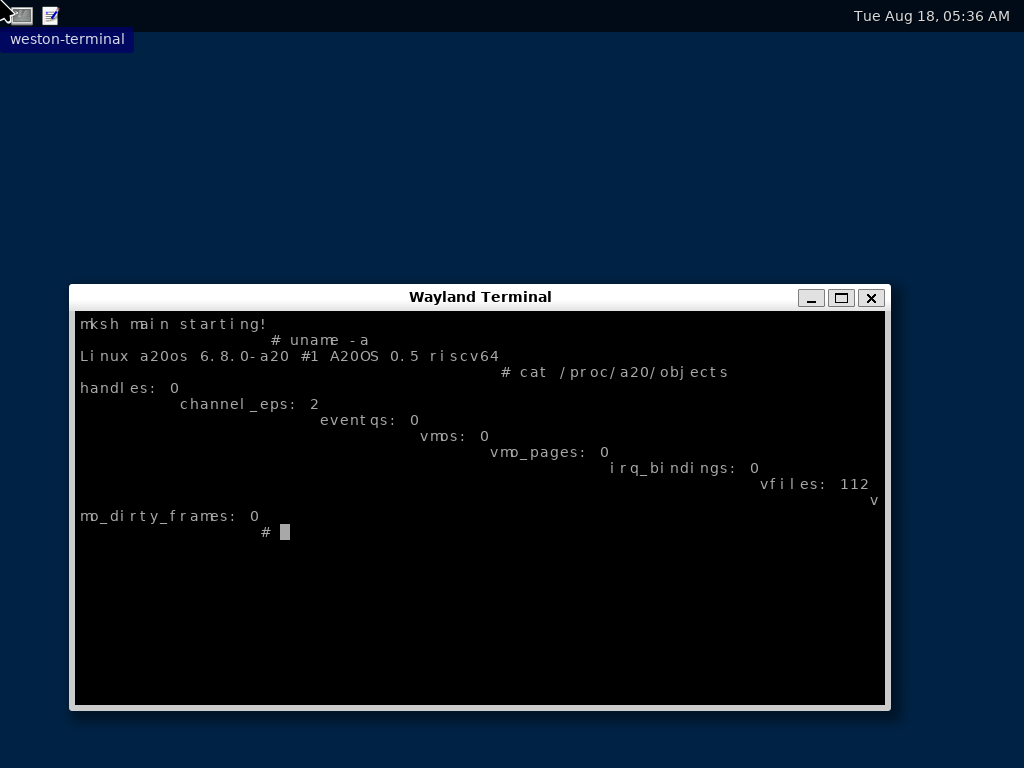
\includegraphics[width=\linewidth]{desktop-riscv64.png}
            \end{tcolorbox}
            \vspace{-0.3em}
            \srcnote{实拍：riscv64 QEMU（virtio-gpu + virtio-input）运行 Weston (Wayland) 桌面；终端内 \code{uname} 显示 \code{A20OS 0.5 riscv64}。}
        \end{column}
    \end{columns}
\end{frame}

\begin{frame}{更多运行实拍（预留位）\framesubtitle{把对应文件名的 PNG 放进 docs/slides/figures/ 重新编译，占位框自动替换为真图}}
    \begin{columns}[t]
        \begin{column}{0.48\textwidth}
            \shotslot{lvgl-desktop.png}{LVGL 自研桌面：仪表盘 / 终端 / 文件 / 网络 / 进程监控}
            \vspace{0.15em}
            \shotslot{virgl-3d.png}{virtio-gpu virgl 3D 加速（\code{gpu3d\_test} / glxgears）}
        \end{column}
        \begin{column}{0.48\textwidth}
            \shotslot{distro-xfce.png}{Alpine 发行版 XFCE 会话（\code{make distro-run}）}
            \vspace{0.15em}
            \shotslot{visionfive2-real.png}{星光 2 / 龙芯 LS2K1000 真机运行}
        \end{column}
    \end{columns}
\end{frame}

\begin{frame}{内核 DRM 强化与 3D 图形加速}
    \begin{columns}[t]
        \begin{column}{0.5\textwidth}
            \begin{block}{内核 DRM 强化}
                \footnotesize
                \begin{itemize}
                    \item \high{唯一 KMS 对象 ID}：plane / crtc / connector / encoder 互不冲突
                    \item 页翻转事件：FIFO 不覆盖、seq 单调、时间戳单调钟、\code{EBUSY} 语义
                    \item 标准 32 字节 UAPI 结构，杜绝栈溢出
                    \item EDID blob property（含合成合规 EDID）
                \end{itemize}
            \end{block}
        \end{column}
        \begin{column}{0.47\textwidth}
            \begin{block}{3D：virtio-gpu virgl}
                \footnotesize
                \begin{itemize}
                    \item \high{内核 3D 命令路径完整}：feature 协商、capset、context / resource / submit 透传
                    \item 渲染在宿主机，guest 内核只搬运命令与资源
                    \item \code{A20\_GPU\_IOCTL\_*} 经 \code{/dev/dri/card0} 暴露
                    \item 与 2D fbdev 路径互不干扰，无 virgl 自动回退
                \end{itemize}
            \end{block}
        \end{column}
    \end{columns}
    \vspace{0.3em}
    \srcnote{3D 链路：用户态 $\rightarrow$ \code{ioctl(/dev/dri/card0)} $\rightarrow$ \code{drm\_ioctl} $\rightarrow$ \code{gpu\_ioctl} $\rightarrow$ \code{SUBMIT\_3D} $\rightarrow$ virglrenderer $\rightarrow$ 宿主 GPU；自测工具 \code{gpu3d\_test}}
\end{frame}

\begin{frame}{发行版 rootfs 直跑：拿 A20OS 当发行版的内核}
    \begin{columns}[t]
        \begin{column}{0.55\textwidth}
            \footnotesize
            \begin{itemize}
                \item \code{make distro-run}：构建内核 + 包管理器拉取\high{原生 Alpine} rootfs + 启动 QEMU (GUI)
                \item 磁盘布局：\code{fat32.img}（自研用户态）+ \code{rootfs.img}（发行版）
                \item init 检测 \code{a20-distro} 标记后 \code{chroot} 进入发行版，由\high{发行版自身的 stage-2 init} 编排桌面会话
                \item 内核补齐发行版需要的全部行为：netlink uevent、\code{PR\_SET\_PDEATHSIG}、\code{/sys/dev/char}、DRM 能力位、evdev ABI
            \end{itemize}
            \vspace{0.2em}
            \srcnote{关键文件：\code{user/rootfs/alpine/}、\code{user/init.c}；文档 \code{docs/distro/}}
        \end{column}
        \begin{column}{0.42\textwidth}
            \begin{a20warnbox}
                \footnotesize 理念：“优先在内核实现，而不是删依赖”——distro 路径没有改组件的自由，内核要么行为到位，要么桌面起不来。
            \end{a20warnbox}
        \end{column}
    \end{columns}
\end{frame}

% ==================================================
\renewcommand{\azsectionsummary}{%
    面向 BuildStorm 热区的 14 项优化全部保留真实计时；%
    双架构 BuildStorm 2551/2315 s $\rightarrow$ 1483/1399 s，用例 180/180 全过。}
\section{性能}

\begin{frame}{性能优化体系（面向 BuildStorm 热区）}
    \begin{columns}[t]
        \begin{column}{0.58\textwidth}
            \footnotesize
            \begin{itemize}
                \item \high{用户 vDSO}：riscv64 / loongarch64 \code{clock\_gettime} 零陷阱
                \item \high{COW 页错误 TLB 定向失效}：广播 SBI/IPI $\rightarrow$ 只向 \code{mm->active\_cpus} 定向
                \item \high{批量延迟 frame 释放}：\code{frame\_put\_many} 每 64 帧只取一次 \code{pfa.lock}
                \item \high{ext4 命名空间读写锁}：8 个 rustc 的 dcache 查找不再互斥
                \item \high{VMA 索引 256 $\rightarrow$ 1024}：编译器进程保持 O(log n) 二分
                \item \high{PRIVATE futex 跳过页表遍历}；fault 去冗余检查
                \item per-vnode 共享映射开关 + 热路径索引化，消除全局脏页扫描
            \end{itemize}
        \end{column}
        \begin{column}{0.39\textwidth}
            \begin{a20keybox}
                \footnotesize\textbf{方法论}\par
                \vskip0.2em
                每项保留真实计时；数字只按干净提交固定，不外推。
            \end{a20keybox}
            \vspace{0.3em}
            \srcnote{文档：\code{docs/BuildStorm-2026.md}；mm/futex/sched 等全组压力验证}
        \end{column}
    \end{columns}
\end{frame}

\begin{frame}{决赛 BuildStorm：双架构 180/180，耗时下降约 40\%}
    \begin{columns}[t]
        \begin{column}{0.56\textwidth}
            \begin{tikzpicture}[baseline={(current bounding box.north)}]
                \begin{axis}[
                    xbar, bar width=5.5pt,
                    width=0.98\linewidth, height=5.2cm,
                    symbolic y coords={Linux 基线, 决赛快照, 第一批优化, 优化前},
                    ytick=data,
                    xmin=0, xmax=3100,
                    xlabel={BuildStorm elapsed (s)}, xlabel style={font=\scriptsize},
                    xmajorgrids, major grid style={a20navy!10},
                    axis line style={draw=none}, tick style={draw=none},
                    yticklabel style={font=\tiny},
                    xticklabel style={font=\tiny, color=a20gray},
                    legend style={font=\tiny, draw=none, at={(0.98,0.30)}, anchor=east, legend columns=1},
                    nodes near coords, every node near coord/.append style={font=\tiny, color=a20gray},
                ]
                    \addplot[xbar, fill=a20blue, draw=none] coordinates {(2551,优化前) (1966,第一批优化) (1483,决赛快照) (638,Linux 基线)};
                    \addplot[xbar, fill=a20accent, draw=none] coordinates {(2315,优化前) (1884,第一批优化) (1399,决赛快照) (565,Linux 基线)};
                    \legend{RISC-V64, LoongArch64}
                \end{axis}
            \end{tikzpicture}
            \srcnote{快照 d5ae5a16 / f3e3ce48 / f9732348，同一 workload、8 vCPU、TCG multi；与 Linux 基线跨 QEMU 版本，按各自证据边界解释。}
        \end{column}
        \begin{column}{0.41\textwidth}
            \statcard[0.98\linewidth]{-41.9\% / -39.6\%}{RV / LA 相对优化前耗时下降}
            \vspace{0.25em}
            \statcard[0.98\linewidth]{180/180}{BuildStorm 用例通过（双架构）}
            \vspace{0.25em}
            \statcard[0.98\linewidth]{199.10/200}{CAgent 得分（10/10 通过）}
            \vspace{0.25em}
            \srcnote{决赛快照 \code{f9732348}：exit 0 主动关机，产物 SHA-256 存档。}
        \end{column}
    \end{columns}
\end{frame}

% ==================================================
\renewcommand{\azsectionsummary}{%
    混合驱动模型：零开销 MMIO + 统一 hwapi + 双部署 profile；%
    drvmod 可加载模块约 80 个导出符号唯一 API 面；下至 64 KiB SRAM 的 MCU。}
\section{驱动与平台}

\begin{frame}{混合驱动模型}
    \begin{itemize}
        \item \high{零开销 MMIO}：板级地址用宏内联，\code{readl/writel} 编译为单条 load/store
        \item \high{统一 hwapi}：\code{request\_irq}、\code{dma\_alloc}、\code{clock\_get\_cycles} 跨架构抽象
        \item \high{类 ops vtable}：\code{block\_dev\_ops\_t}、\code{net\_dev\_ops\_t}、\code{char\_dev\_ops\_t}
        \item 编译期注册：\code{DRIVER\_REGISTER} / \code{BOARD\_REGISTER} 放入 \code{.driver\_init} linker section
        \item 双部署 profile：\code{generic}（DriverStore + \code{.a20drv}）/ \code{embedded}（静态链接，决赛默认）
        \item drvmod：ET\_REL 装载 + \code{.a20drv} 描述段 + veneer/GOT，\high{约 80 个导出符号}唯一 API 面
    \end{itemize}
    \vspace{0.3em}
    \srcnote{关键文件：\code{docs/drivers/README.md}、\code{kernel/include/drivers/hwapi.h}；验证 \code{make smoke-drvmod}}
\end{frame}

\begin{frame}{设备生态：音频 / USB / PCI / 虚拟机}
    \begin{columns}[t]
        \begin{column}{0.5\textwidth}
            \begin{block}{音频子系统}
                \footnotesize
                virtio-snd · Intel HDA（PCI class 驱动，CODEC 拓扑发现）· PC Speaker；\code{/dev/audioN} + capability/format 校验；\code{audioplay} 与 FFmpeg 播放器
            \end{block}
            \begin{block}{USB 协议栈}
                \footnotesize
                host / class / core 分层；xHCI；HID / 存储类；\code{make smoke-usb-x86\_64}
            \end{block}
        \end{column}
        \begin{column}{0.47\textwidth}
            \begin{block}{PCI 与平台设备}
                \footnotesize
                ECAM 枚举 · \high{e1000 真 PCI 网卡} · ahci · virtio-scsi · 平台网卡（starfive\_gmac / ls2k\_gmac）· dw\_sdio
            \end{block}
            \begin{block}{VirtualBox}
                \footnotesize
                x86\_64 / aarch64 经 \high{UEFI + ACPI + ECAM} 引导；VMSVGA / E1000 / VirtIO-SCSI
            \end{block}
        \end{column}
    \end{columns}
\end{frame}

\begin{frame}{嵌入式与 MCU：同一内核，64 KiB SRAM 起步}
    \begin{columns}[t]
        \begin{column}{0.5\textwidth}
            \begin{block}{STM32F103（ARMv7-M / NOMMU）}
                \begin{itemize}
                    \item 64 KiB Flash / 20 KiB SRAM bring-up（QEMU 验证）
                    \item 普中玄武 ZET6：512 KiB Flash / 64 KiB SRAM
                    \item 外设：LCD、舵机 / 执行器、DHT11 传感器、蓝牙、ESP8266、背光
                \end{itemize}
            \end{block}
        \end{column}
        \begin{column}{0.47\textwidth}
            \begin{block}{PPC64LE}
                QEMU pSeries 固件，MMU 单核边界
            \end{block}
            \begin{block}{跨平台工程}
                统一 arch/HAL 抽象、七架构构建矩阵，物理板与虚拟平台同构验证。
            \end{block}
        \end{column}
    \end{columns}
    \vspace{0.3em}
    \srcnote{入口：\code{make stm32f103-bringup}、\code{make stm32f103-xuanwu}、\code{make run-stm32f103-qemu}、\code{make ARCH=ppc64le run}}
\end{frame}

% ==================================================
\renewcommand{\azsectionsummary}{%
    54 项行为冒烟门禁 + 15 项静态/运行时审查门禁；%
    文档即事实契约保证设计与实现不漂移；/proc/a20 暴露运行时对象与调度计数。}
\section{工程化与验证}

\begin{frame}{测试门禁体系：54 项冒烟全部可复现}
    \begin{columns}[t]
        \begin{column}{0.55\textwidth}
            \begin{tikzpicture}[baseline={(current bounding box.north)}]
                \begin{axis}[
                    a20bar, width=0.97\linewidth, height=5.6cm,
                    enlarge y limits=0.09,
                    symbolic y coords={网络套件, 时钟/输入, IOMMU/驱动隔离, GUI 行为判帧, Linux ABI 语义, 架构启动/矩阵, 并发与压力, Native ABI 专项},
                    ytick=data,
                    xmax=19,
                    nodes near coords,
                ]
                    \addplot[xbar, fill=a20blue, draw=none] coordinates {
                        (16,Native ABI 专项) (12,并发与压力) (9,架构启动/矩阵)
                        (7,Linux ABI 语义) (5,GUI 行为判帧) (2,IOMMU/驱动隔离)
                        (2,时钟/输入) (1,网络套件)};
                \end{axis}
            \end{tikzpicture}
            \srcnote{54 项 \code{make smoke-*} 按类别分布；明细见备查 D。}
        \end{column}
        \begin{column}{0.42\textwidth}
            \statcard[0.98\linewidth]{54}{\code{make smoke-*} 行为冒烟门禁}
            \vspace{0.25em}
            \statcard[0.98\linewidth]{61}{项 \code{check-*} 审查 / 构建门禁}
            \vspace{0.25em}
            \statcard[0.98\linewidth]{30+}{自研压力 / 语义测试工具（\code{user/cmds}）}
            \vspace{0.25em}
            \srcnote{调度压力矩阵 \code{check-proc-step8-local}：双架构 1 核 / 8 核累计。}
        \end{column}
    \end{columns}
\end{frame}

\begin{frame}{文档即事实 + 可观测性}
    \begin{columns}[t]
        \begin{column}{0.52\textwidth}
            \footnotesize
            \begin{itemize}
                \item \code{DOCS\_AS\_FACT\_CONTRACT}：架构文档描述\high{当前实现}，未来设计放规划材料
                \item 20+ 静态审查门禁：锁模型、ABI 边界、I/O 进展模型、文档漂移等
                \item 外部依赖边界审查（musl / lwIP / 用户态工具）
                \item Docker 交叉编译环境 + 可选 \code{ccache}
                \item 92 篇设计文档、1.6 万行，随代码同仓演进
            \end{itemize}
        \end{column}
        \begin{column}{0.45\textwidth}
            \begin{a20keybox}
                \footnotesize\textbf{\code{/proc/a20/} 运行时状态面}\par
                \vskip0.2em
                \begin{itemize}
                    \item \code{objects}：7 项实时对象计数 + 句柄硬配额审计
                    \item \code{task\_lifetime}：task/ref、runqueue、wait/wake、timeout、migration、IPI、violation 计数
                    \item \code{sched\_base\_slice}：EEVDF 虚拟 slice 旋钮
                \end{itemize}
            \end{a20keybox}
        \end{column}
    \end{columns}
    \vspace{0.3em}
    \srcnote{崩溃 / 重启循环后对象计数回归基线，泄漏审计可重复验证。}
\end{frame}

% ==================================================
\renewcommand{\azsectionsummary}{}
\section{未来工作}

\begin{frame}{下一步工作}
    \begin{enumerate}
        \item \high{I/O 完全事件驱动}：收敛块 / 网络设备最后的轮询 fallback 路径
        \item \high{网络栈深化}：降低 \code{g\_lwip\_lock} 竞争，扩展 socket 并发测试
        \item \high{VFS / Linux ABI 语义收紧}：\code{partial} $\rightarrow$ \code{full} 逐组提升
        \item \high{IOMMU 动态 DMA}：per-device domain 与 fault 队列消费，端到端硬件隔离
        \item \high{Native 多架构矩阵}：将 16 项原生测试扩展至全架构 CI-like 运行
    \end{enumerate}
    \vspace{0.5em}
    \begin{a20keybox}
        \small 核心追求：在保证 Linux 生态兼容的前提下，构建更安全、更高性能、更可维护的下一代内核底座。
    \end{a20keybox}
\end{frame}

% ==================================================
% 致谢
\section*{}
\begin{frame}[plain]
    \begin{tikzpicture}[remember picture, overlay]
        \fill[a20navy] (current page.north west) rectangle (current page.south east);
        \node[anchor=center, text=white!20!a20navy, font=\fontsize{56}{56}\bfseries\selectfont]
            at ([yshift=1.1em]current page.center) {Q \& A};
        \node[anchor=center, text=white, font=\Large\bfseries]
            at ([yshift=-1.6em]current page.center) {感谢各位专家评委，恳请批评指正};
        \node[anchor=center, text=a20light!75, font=\footnotesize, align=center]
            at ([yshift=-3.6em]current page.center)
            {感谢全国大学生计算机系统能力大赛平台 · 感谢开源社区 AOSC、plos-clan 的支持\\[0.3em]
             \ttfamily\scriptsize gitlab.eduxiji.net/T202610486999803/oskernel2025-a20 ~~|~~ github.com/fQwQf/A20OS};
        \node[anchor=north east]
            at ([xshift=-1em,yshift=-0.8em]current page.north east)
            {
\includegraphics[width=0.14\paperwidth]{a20os-logo-white.pdf}};
    \end{tikzpicture}
\end{frame}

% ==================================================
% 附录：答辩备查（不进目录）
\appendix

\begin{frame}{备查 A：EEVDF 正确性与参数}
    \begin{columns}[t]
        \begin{column}{0.55\textwidth}
            \footnotesize
            \begin{itemize}
                \item 权重表 \code{sched\_prio\_to\_weight[40]} 与 Linux 同源：nice $-20 \rightarrow 43020$，nice $+19 \rightarrow 88$
                \item \code{EEVDF\_NICE0\_LOAD = 1024}，基准 slice 10 ms，\code{EEVDF\_MAX\_LAG} 10 ms
                \item eligibility：$\mathrm{vruntime} \le \mathrm{vtime}$；pick：eligible 中最小 deadline
                \item 延迟唤醒补偿按 lag 计入 vruntime，但钳制到 MAX\_LAG，防止“睡一次吃光 CPU”
            \end{itemize}
        \end{column}
        \begin{column}{0.42\textwidth}
            \begin{a20keybox}
                \footnotesize\textbf{可能被问：与 Linux EEVDF 的差异}\par
                \vskip0.2em
                数据结构为 per-CPU 队列 + 显式所有权状态机，非 rbtree 全局队列；RT 单独级 0 恒优先；slice 经 \code{/proc/a20/sched\_base\_slice} 运行时可调，用于桌面 / HPC 形态切换。
            \end{a20keybox}
            \vspace{0.3em}
            \srcnote{证据：\code{kernel/proc/sched.c}、\code{kernel/proc/proc\_internal.h}、\code{docs/eevdf-scheduler.md}}
        \end{column}
    \end{columns}
\end{frame}

\begin{frame}{备查 B：并行编译崩溃的根因与修复}
    \footnotesize
    \begin{itemize}
        \item \high{现象}：8 核 / 8 job 全量 cargo 编译下，RISC-V64 rustc ICE；LoongArch64 SIGILL / SIGSEGV / 地址异常
        \item \high{根因}：清除或替换 PTE 后，旧 frame / page-cache 引用可能在\high{远端 TLB shootdown 完成前}被释放并复用——新写入落到旧物理页
        \item \high{修复}：per-mm TLB invalidation transaction，旧 backing 延迟到 shootdown 确认后释放；LoongArch64 同步等待远端 shootdown；统一 VMA deferred flush、slab、block-cache、buddy 的并发边界
        \item \high{另两处持久化损坏}：VirtIO packed used ring 16 位 \code{idx} 撕裂读（固定布局 + barrier）；block-cache 并发写回旧 ext4 bitmap 晚于新快照落盘（writeback/fill 锁 + dirty generation 定序）
    \end{itemize}
    \vspace{0.3em}
    \srcnote{完整分析与证据边界：\code{docs/BuildStorm-2026.md} §2；验证：并发 rustc + 官方测试组 + 定点 probe 交叉验证}
\end{frame}

\begin{frame}{备查 C：361 / 139 的统计口径}
    \begin{columns}[t]
        \begin{column}{0.55\textwidth}
            \footnotesize
            \begin{itemize}
                \item Linux ABI：\code{syscall\_table.def} 注册 \high{361 个调度项}（含 2 个 A20 扩展、5 个 x86\_64 legacy 槽），每个注册项都有真实 handler
                \item 少数 \code{-ENOSYS} 返回是 Linux 本身的架构 / 版本正确语义（如 \code{nfsservctl} 已于 Linux 4.19 移除）
                \item 语义等级逐区标注 full / partial，见 \code{syscall\_coverage.md}，不夸大兼容度
                \item Native ABI：\code{syscall\_table.def} 中 139 条 X-macro 注册
            \end{itemize}
        \end{column}
        \begin{column}{0.42\textwidth}
            \begin{a20keybox}
                \footnotesize\textbf{验证方法}\par
                \vskip0.2em
                \code{make smoke-abi-linux} 逐组语义验证；\code{smoke-syscall-ext} 覆盖 io\_uring / landlock / userfaultfd / perf 等现代机制；真实负载：Alpine 发行版 + Cargo 全量编译。
            \end{a20keybox}
        \end{column}
    \end{columns}
\end{frame}

\begin{frame}{备查 D：54 项冒烟门禁明细}
    \begin{table}
        \centering
        \scriptsize
        \renewcommand{\arraystretch}{1.18}
        \begin{tabular}{cll}
            \toprule
            \textbf{数量} & \textbf{类别} & \textbf{目标} \\
            \midrule
            16 & Native ABI 专项 & \code{smoke-native-\{contract,deepen,ext,futex,ipc,} \\
               & & \code{isolation,linux,mm,registry,rtcd,shmring,svc,ubd,…\}} \\
            12 & 并发与压力 & \code{\{mm,sched,futex,vfs,proc,procfs,pty,scm,signalfd,evdev\}-stress} 等 \\
            9 & 架构启动 / 矩阵 & \code{smoke-<arch>} × 7 + \code{smp-bringup} + \code{arch-mmu-matrix} \\
            7 & Linux ABI 语义 & \code{abi-linux}、\code{syscall-ext}、\code{ptrace}、\code{proc-a20}、\code{vfs-edge} 等 \\
            5 & GUI 行为判帧 & \code{smoke-qemu-gui-\{riscv64,loongarch64,aarch64,x86\_64,arm32\}} \\
            2 & IOMMU / 驱动隔离 & \code{iommu-discovery}、\code{iommu-udriver-isolation} \\
            2 & 时钟 / 输入 & \code{clock-vdso}、\code{dual-input} \\
            1 & 网络套件 & \code{smoke-network-suite}（TCP/UDP/ICMP/DNS/AF\_UNIX） \\
            \bottomrule
        \end{tabular}
    \end{table}
    \vspace{0.2em}
    \srcnote{全部经 \code{make smoke-*} 一键复现；超时无 PASS 标记即失败（行为判据，非仅编译通过）。}
\end{frame}

\end{document}
